\documentclass[runningheads]{llncs}

\usepackage[utf8]{inputenc}
\usepackage[T1]{fontenc}
\usepackage{graphicx}
\usepackage{array}
\usepackage{booktabs}
\usepackage{amsmath,amssymb}
\usepackage{algorithm}
\usepackage{algorithmic}
\usepackage{float}
\usepackage{microtype}

\raggedbottom
\emergencystretch=3em

\begin{document}

\title{IAGAPC-Enhanced: Kinematically Feasible Genetic Trajectory Optimization for Mobile-Sink Wireless Sensor Networks}
\titlerunning{Kinematically Feasible GA Trajectories for Mobile-Sink WSNs}

\author{Masapeta Kuruva Bhargava Sri Sai \and Rapaka Vikranth \and Radhika N. \and Radhika G.}
\authorrunning{Sri Sai et al.}
\institute{Department of Computer Science and Engineering, Amrita School of Computing, Coimbatore, Amrita Vishwa Vidyapeetham, India \\
\email{cb.sc.u4cse24268@cb.students.amrita.edu}, \email{cb.sc.u4cse24244@cb.students.amrita.edu}, \email{n\_radhika@cb.amrita.edu}, \email{g\_radhika@cb.amrita.edu}}

\maketitle
\begin{abstract}
Wireless sensor networks (WSNs) are equipped with limiited resources,hence efficient use of energy is needed to increase lifespan of network.Inculcation of mobile sink to deal with energy issues improves the lifetime of the network. Mobile-sink
trajectory planning is usually optimized for spatial coverage alone. It
rarely asks whether the resulting path is the one a physical sink could execute
efficiently. We propose IAGAPC-Enhanced (Improved Adaptive Genetic
Algorithm with Path Compactness, Enhanced), a genetic algorithm that layers
Catmull-Rom spline densification and an explicit kinematic-feasibility
constraint onto adaptive operator control and a diversity-restart
mechanism. Five baselines meet it on common ground: an adaptive-parameter
GA, a tabu-search hybrid, an artificial-bee-colony hybrid, a distributed
island-model GA, and a cluster-first K-means/TSP scheme. All six share one
LEACH-style clustering and multi-hop relay substrate in ns-3.45, with ten
random-initialization runs per scheme with confidence intervals called seeds. Across this evaluation,
IAGAPC-Enhanced's trajectories turns substantially less deeper than every
baseline's (22.99$^\circ$ vs. 74.81--109.89$^\circ$, non-overlapping 95\%
confidence intervals). This is the one result our data separates cleanly.
Packet delivery ratio, throughput, delay, and energy efficiency do not
separate between schemes at this sample size. We report that directly
rather than  ranking the data does not support. Absolute delivery
performance is low across all six schemes. We trace to PHY-layer
contention among 200 nodes sharing a WiFi-modeled channel. We disclose that
channel as a deviation from the IEEE 802.15.4 system model, not as
equivalent to it.
\end{abstract}


\keywords{wireless sensor networks \and mobile sink \and genetic algorithm \and trajectory optimization \and cluster-head election \and kinematic feasibility}
\section{Introduction}
\label{sec:intro}

A wireless sensor network (WSN) with a single static base station forces
nodes near that station to relay traffic for the rest of the field. Those
nodes exhaust their batteries first. This is the well-documented
energy-hole problem. Introducing a mobile sink that physically visits the
deployment area redistributes this load, but it converts a routing problem
into a motion-planning problem. The sink's trajectory now directly
determines how much of the network it can service, and how often, before
energy reserves run out.

Much of the literature settles the trajectory independently of the
clustering and routing layer beneath it, or optimizes the path for spatial
coverage alone. Either way, it never asks whether the resulting sequence of
moves is something that a physical platform could execute. Geometric validity is
not executability: sharp direction reversals burn travel time.Every
second spent turning is a second the sink collects nothing,that cost shows
up in the network's energy budget and not the path length.

This paper targets that gap. We propose IAGAPC-Enhanced, a genetic
algorithm for mobile-sink trajectory planning and combining adaptive
crossover/mutation control, a diversity-restart operator, Catmull-Rom
spline densification, and has explicit kinematic-feasibility constraint
tying waypoint timing to the sink's maximum velocity. We evaluate it
against five baseline trajectory strategies representative of prior
GA-based WSN work: an adaptive-parameter GA, a tabu-search hybrid, an
artificial-bee-colony hybrid, a distributed island-model GA, and a
cluster-first K-means/TSP scheme. All six run under one shared two-tier
architecture: LEACH-style cluster-head election beneath the
sink-trajectory layer, with greedy geographic multi-hop relay to the
nearest live cluster head.

Our contributions are:
\begin{itemize}
\item A kinematically-constrained GA trajectory planner
      (IAGAPC-Enhanced) that produces markedly smoother sink paths than five
      comparably-structured baselines, evaluated under identical simulation
      conditions in all six cases.
\item A ten-seed, six-scheme energy-efficiency comparison reported
      honestly as statistically inconclusive where the data supports no
      ranking, rather than a single favorable number presented without its
      overlapping confidence intervals.
\item A fully instrumented ns-3 evaluation harness for six trajectory
      schemes sharing clustering/relay substrate, together with an
      explicit accounting of where the link layer, not the trajectory
      algorithm. This is the limiting factor for absolute delivery performance at
      this deployment scale.
\end{itemize}

Section~\ref{sec:related} surveys related work by layer; Section~\ref{sec:model}
states the network and energy model; Section~\ref{sec:method} develops
IAGAPC-Enhanced; Section~\ref{sec:setup} details the simulation; results
and conclusion follow in Sections~6--7.

\section{Related Work}
\label{sec:related}

Genetic algorithms enter WSN design at several distinct layers, and we
group prior work by layer rather than walk through.

A large share of
this literature keeps the sink fixed and applies a GA to cluster-head
selection or intra-network routing: encoding the whole
source-to-sink route as a chromosome~\cite{kowsalya2020cdarga}, weighing
hop distance against residual energy in the fitness
function~\cite{muthukkumar2022gaemc}, splitting sleep-scheduling and
clustering into two sequential GA passes~\cite{abbas2025twophase}, or
layering a trust score onto adaptive-GA routing for attack
resilience~\cite{han2022taga}. B.D. Bala, H.M. Hassan, and S.M. Lawan~\cite{bala2024leachm} report a
bacterial-conjugation operator beating a GA at the same clustering task in
their setting. That is a reminder that genetic search is one viable
metaheuristic here, not an automatic winner. G. Radhika and N.
Radhika~\cite{radhikag2025qlearning} replace GA-based election by
pairing attribute-based cluster-head selection with a Q-learning routing
algorithm embedded with action sequences. Adaptive Coati Optimization step tunes the algorithm's action
sequences to keep nodes from going unreachable. Their comparison is against
three ablations of that same design: the optimized learner stripped of
clustering, and the untuned learner run both with and without the result. These results 
report an 11.82\% throughput gain and a 25.19\% cut in
energy consumption. None of this group moves the sink.

N.a. Mottaki, H. Motameni,
and H. Mohamadi~\cite{mottaki2023hybridga}, A.K. Idrees and W.L.
Al-Yaseen~\cite{idrees2021digalco}, S. Sun, Y. Chen, and L.
Dong~\cite{sun2024garwoa}, A. Somauroo and V.
Bassoo~\cite{somauroo2019pegga}, and Varsha, M. Bala, M. Kumar, and N.
Kumar~\cite{varsha2019tabuga} all use a GA to decide which deployed sensors
stay active rather than to cluster or route. Their approaches include
hybridizing tabu search into coverage-set scheduling, distributing election
across virtual subregions, pairing a GA with reinforced whale-optimization
for pure coverage, and replacing PEGASIS's greedy chain with a GA-built
one, tracing large lifetime gains to chain geometry specifically (a
structural isolation that parallels what we do with trajectory smoothness).
Varsha, M. Bala, M. Kumar, and N. Kumar route over a three-tier
heterogeneous clustering protocol with a hybrid tabu-GA. 

R. Hamidouche, Z. Aliouat, A.A.A. Ari,
and A. Gueroui~\cite{hamidouche2021mssa} propose work closest to our
problem that optimizes the sink's own path or stop points, steering a
salp-swarm search toward the fullest cluster-head buffer over a fixed
grey-wolf clustering. Another combines Voronoi deployment
with a chaotic-Aquila path planner, beating six baselines on delay,
lifetime, PDR, and throughput at once~\cite{sangeetha2024exaqmspp}. A third
treats itinerary planning as a multi-criteria trade-off, centrally via
IQCQP and distributedly via fuzzy TOPSIS; the gap between the two closes in
dense deployments but opens to 14--26\% (depending on the metric).Once the
site grid thins out~\cite{khalily2023itinerary}. Others place Steiner-tree
sink stops over bio-inspired clustering for a hybrid WSN/LTE
path~\cite{mohan2024mfoms}, and a GA-optimized cluster-head election is done 
explicitly for movable sinks, available to us only as an
abstract~\cite{nandan2021optigachs}. Metaheuristics other than the GA, and
learned policies, have also been aimed at the routing decision itself.
G. Radhika, N. Radhika, and S. Paul~\cite{radhikag2024cooperative} treat congestion as the thing
to avoid scores. Each link with a traffic-density probability, builds an
adaptive Petal Spider Ant Colony clustering over the result to pick stable
next hops, and hand the surviving candidates to a Q-learning route
selector. After which a proactive cluster-routing layer then throttles by a lookup on
duty-cycle energy, spreading load to stretch lifetime. PAR, PSO, and FAPRP
are the yardsticks. Their scheme tops out at 99\% on both routing and
throughput performance with 100 nodes. The observed results are (84\% and 83\% respectively in the
sparse 25-node case). It drops 15\% of packets at 100 nodes and cuts
end-to-end latency from 24\,ms at 25 nodes to 8\,ms at 100. A different
tack appears in G. Radhika and N. Radhika~\cite{radhikag2023smorl}. Every sensor
becomes an agent picking its own next hop by reward, and a spider-monkey
optimization step nominates the candidates it chooses among, scoring them
on residual energy and inter-node distance. Their NS-2 study is anchored on
two baselines, MOSMO and Flock-CC. Against MOSMO they put numbers on
exactly two metrics (latency and control overhead, both down 35\%) and
leave throughput, energy draw, network lifetime, and packet loss as plotted
curves. No report esist pertaining to lifetime and delivery ratio as observed
in the whole group measures. None reports a trajectory-smoothness or
kinematic-feasibility figure we could set beside our own.

G.T. Al-Mamari, F. Bouabdallah, and A.
Cherif~\cite{almamari2025mobilesink} sit
outside the GA-focused corpus entirely. They fix mobile-sink sojourn points
by linear programming and cuckoo search over a grid topology, with an
overhearing-aware energy model as their central contribution and no
clustering or GA involved. We depart from it by placing
trajectory optimization inside a GA framework, comparable operator for
operator against the GA-family baselines above, and by evaluating with a
packet-level simulator rather than an analytical grid model. Two further
gaps shape our design. No paper surveyed here reports an offered-load
sensitivity sweep, and we include one. None uses ns-3 either (NS2, MATLAB,
and OMNeT++ dominate this literature); our choice forces explicit MAC/PHY
contention modeling that an idealized channel would hide. A point
Section~6 returns to. A controlled six-way comparison of distinct GA
\emph{family} structures under one shared network substrate, which is what
we report here, does not appear elsewhere in this corpus.

\section{System Model}
\label{sec:model}

$N$ sensor nodes are deployed uniformly at random over a square field of
side $L$, each tagged normal, advanced, or super. That tier fixes each
node's initial energy budget, so the population is energy-heterogeneous
from round zero. A single mobile sink follows a trajectory computed
offline, before the run begins, as a fixed-length sequence of waypoints.
That trajectory is exactly what the compared optimization procedures
produce. Cluster heads are elected probabilistically every round, in the style of
W.B. Heinzelman, A.P. Chandrakasan, and H.
Balakrishnan~\cite{heinzelman2002leach}: a node $i$ that has not
served as cluster head in the previous $1/p$ rounds computes threshold

\begin{equation}
T(i) = \frac{p}{1 - p \cdot (r \bmod \frac{1}{p})} \cdot \frac{E_{\mathrm{residual}}(i)}{E_{\mathrm{initial}}(i)},
\label{eq:leach}
\end{equation}

\noindent ($p$ = target election probability, $r$ = round index) and becomes
cluster head if a uniform draw falls below $T(i)$, with the residual-energy
factor biasing election away from already-depleted nodes. We chose this
rule for its plainness. Richer alternatives score candidates on link
quality, proximity, and energy jointly before handing routing to a learned
policy~\cite{radhikag2025qlearning}. Keeping election purely probabilistic
instead guarantees that all six compared schemes inherit one identical,
GA-independent clustering layer, so any difference between them traces back
to the trajectory. Ordinary sensors reach their nearest live cluster head by
greedy geographic relay: each hop picks whichever in-range neighbor is
closest to the target, up to a fixed hop cap, and the simulator records a
packet that runs out of forward progress rather than silently discarding
it. Nothing in that hop choice estimates link stability, which is the
quantity that stability-aware relay protocols use to steer around fragile
links~\cite{radhikag2024cooperative}. Distance to the target is our only
criterion. Cluster heads receives and self-generated traffic
to finite, drop-oldest queue, and flushes it to the sink. This is done only when the
sink's trajectory brings it into its range. Figure~\ref{fig:arch} shows the
resulting two-tier architecture.

\begin{figure}[H]
\centering
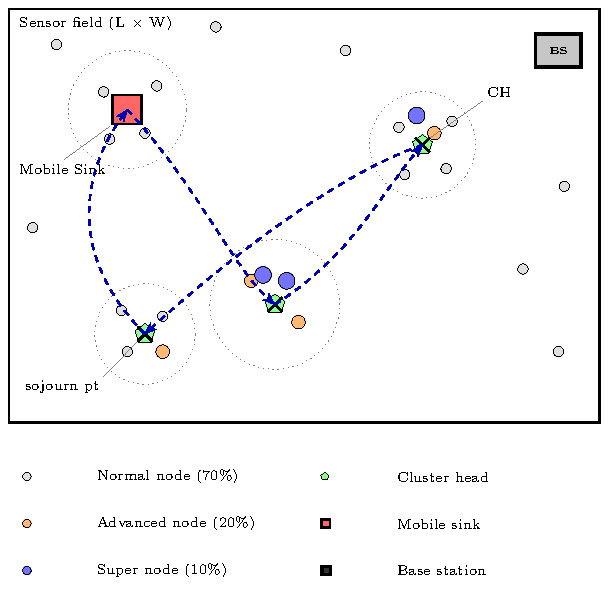
\includegraphics[width=0.7\textwidth]{../figures/architecture-diagram.pdf}
\caption{Two-tier network architecture: ordinary sensor nodes (normal /
advanced / super tiers) reach their nearest live cluster head via greedy
multi-hop relay; cluster heads buffer aggregated traffic until the mobile
sink's trajectory brings it within range.}
\label{fig:arch}
\end{figure}

Radio energy follows a current-draw mode, a fixed current per idle,
receive, transmit, and sleep state, integrated over time spent in that
state at a fixed supply voltage. A node is depleted once cumulative
consumption reaches its tier budget. Radios default to sleep and wake only
on a proximity triggers a cluster head on sink proximity. An ordinary
sensor on the existence of a live route to a cluster head that holds each
sleep/wake window for a fixed duration (Table~\ref{tab:params}). These
window lengths and per-state currents are this study's own configuration
choices, not values drawn from a cited source. Section~6 notes that
this mechanism's isolated contribution to the energy results could not be
validated.

\section{Proposed Methodology: IAGAPC-Enhanced}
\label{sec:method}

IAGAPC-Enhanced optimizes the sink's trajectory as a fixed-length sequence
of $(x,y,t)$ waypoints via a GA with four features on top of a standard GA
loop: adaptive operator rates, a diversity-triggered restart, spline-based
densification, and kinematic-feasibility enforcement. Figure~\ref{fig:flow}
summarizes the pipeline.

\begin{figure}[H]
\centering
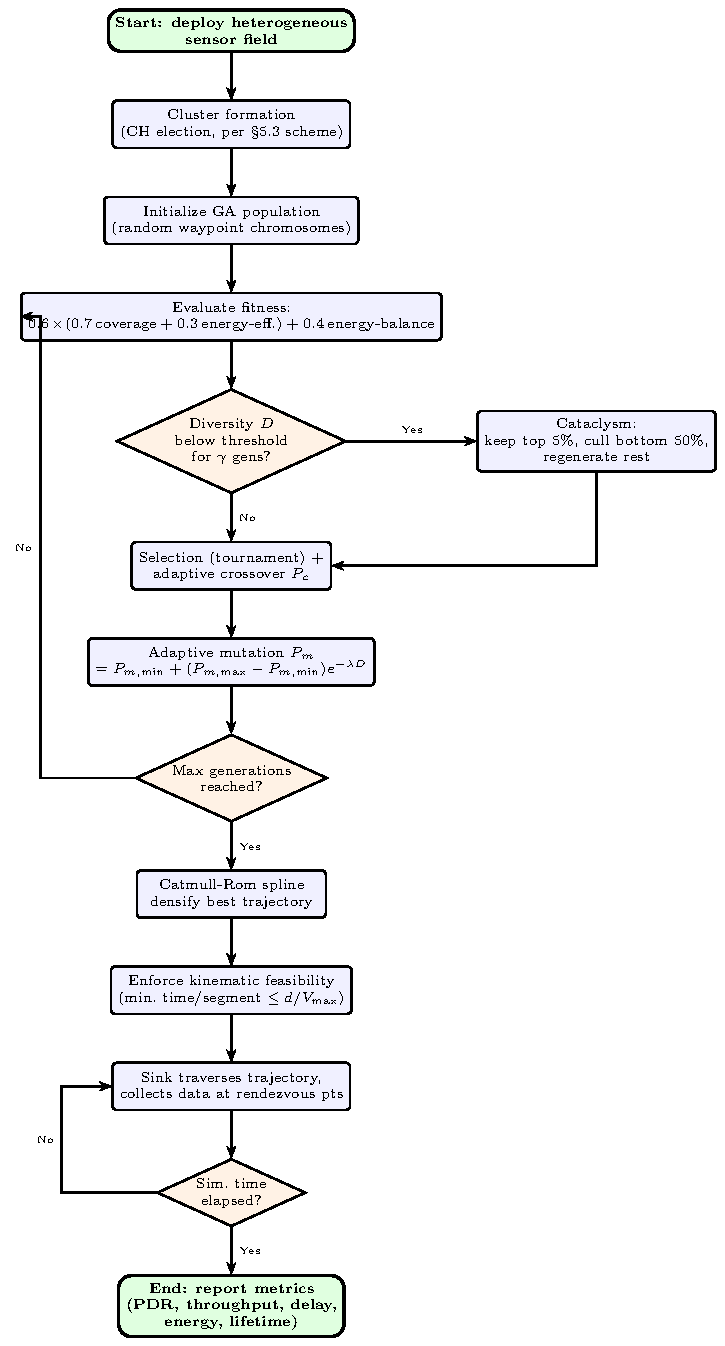
\includegraphics[width=0.5\textwidth]{../figures/flow-diagram.pdf}
\caption{Flow diagram of IAGAPC-Enhanced pipeline.}
\label{fig:flow}
\end{figure}

Fitness combines three terms: coverage (fraction of sensors within range of
some waypoint), path length (shorter total distance), and compactness
(shorter total duration against an a-priori target tour time, estimated
from field geometry and sink speed via a Beardwood-Halton-Hammersley-style
open-tour length). Compactness exists because neither of the other two
terms depends on waypoint timing at all. Without it, nothing penalizes
on visit times drifting toward the edge of their sampling range, and tour
duration grows unbounded.

Each generation, crossover and mutation rates retune from the fitness
spread (best minus average individual): a shrinking spread raises mutation
pressure against premature convergence, a widening one relaxes it. When
population diversity (mean waypoint-to-centroid distance) stays below
threshold for several generations, a Cataclysm operator keeps only the
incumbent best individual and reinitializes the rest, preventing the search
from settling permanently into one basin.

Once the GA converges on control waypoints, Catmull-Rom spline
interpolation inserts intermediate waypoints between each pair, producing a
smoothly curving path instead of a piecewise-linear one. This is the
mechanism directly responsible for Section~6's trajectory-smoothness
result. A final
kinematic-feasibility pass increases any inter-waypoint time gap that would
otherwise require exceeding the sink's maximum velocity. The trajectory
is physically executable, not merely geometrically valid. None of the five
baselines apply this pass, reflecting the same sink-as-point-mass
simplification common across the compared algorithm families.

\section{Simulation Setup}
\label{sec:setup}

Ns-3.45 harness drives all six schemes: clustering, delay, energy, and
traffic behavior are byte-identical across runs (Table~\ref{tab:params}
gives the configuration). And only the trajectory-optimization procedure
changes. One deviation from the system model is stated plainly rather than
folded into the table: the implementation uses ns-3's \texttt{WifiHelper}
(IEEE 802.11) as the link layer, while Section~\ref{sec:model} follows the
IEEE 802.15.4 class in its range/rate assumptions. Deviation
between implementation and specification, not presented as equivalent to
it, whose measured effect on delivery is quantified in Section~6.

\begin{table}[H]
\centering
\caption{Simulation parameters.}
\label{tab:params}
\small
\begin{tabular}{@{}l>{\raggedright\arraybackslash}p{6.9cm}@{}}
\toprule
Parameter & Value \\
\midrule
Simulator & ns-3.45 \\
Deployment area & 1000\,m $\times$ 1000\,m \\
Node count & Harness supports 100, 200, 300, 500; Section~6 results are $n{=}200$ only \\
Node distribution & Uniform random \\
Energy tiers & 0.5\,J / 1.0\,J / 1.5\,J at 70\% / 20\% / 10\% of nodes \\
Link layer & IEEE 802.11b (\texttt{WifiHelper}), see deviation note above \\
Link data rate (PHY) & 1\,Mbps \\
Simulated time per run & $3\times$ a-priori tour-time target \\
Sensing-generation rate & 1 packet / node / 10\,s, fixed \\
Application payload & 512\,B per packet \\
Sensor-to-cluster-head range & 50\,m \\
Cluster-head-to-sink range & 100\,m \\
Cluster-head election probability $p$ & 0.05  \\
Relay hop cap & 3 \\
Sink velocity & 10\,m/s  \\
Duty-cycle check interval & 1.0\,s \\
Duty-cycle wake window & 0.3\,s on proximity trigger \\
GA population size & 50 \\
GA generations & 50 \\
GA waypoints & 8 \\
Seeds per configuration & 10 \\
\bottomrule
\end{tabular}
\end{table}

\section{Results and Discussion}
\label{sec:results}

All results below come from a single frozen configuration ($n{=}200$
nodes, 10 independent seeds per scheme, six schemes, base parameters from
Table~\ref{tab:params}) runs after every fix described in
Section~\ref{sec:setup} was in place. No result in this section predates
that configuration. Reported intervals mean $\pm$ 95\% confidence
interval across the 10 seeds.

\subsection{Trajectory Smoothness}

Table~\ref{tab:turning} reports the average absolute turning angle between
consecutive trajectory segments. The geometric smoothness metric
directly targeted by IAGAPC-Enhanced's spline densification and
kinematic-feasibility pass. This is also the one metric in our evaluation
that is purely a function of the waypoint geometry. Each scheme outputs does not depend on the network, MAC, or PHY layer at all, which is why it
is the result we treat as primary.

\begin{table}[t]
\centering
\caption{Average turning angle by scheme (degrees, mean $\pm$ 95\% CI, $n{=}200$, 10 seeds).}
\label{tab:turning}
\begin{tabular}{lc}
\toprule
Scheme & Turning angle ($^\circ$) \\
\midrule
IAGAPC-Enhanced & \textbf{22.99 $\pm$ 1.67} \\
CGAPD & 74.81 $\pm$ 8.23 \\
EGATS-N & 83.97 $\pm$ 12.39 \\
AGAPC & 88.41 $\pm$ 13.62 \\
DGA-M & 90.66 $\pm$ 9.50 \\
RCGA-ABC & 109.89 $\pm$ 15.23 \\
\bottomrule
\end{tabular}
\end{table}

IAGAPC-Enhanced's confidence interval does not overlap any baseline's that narrow gap is to CGAPD, whose mean sits more than 45$^\circ$ away, with
no shared range.
The mechanism is directly attributable to the spline-densification and
kinematic-feasibility steps described in Section~\ref{sec:method}. No
other scheme applies either, and no other scheme comes close to this
result. This is the cleanest, most reproducible finding in our evaluation.

\begin{figure}[H]
\centering
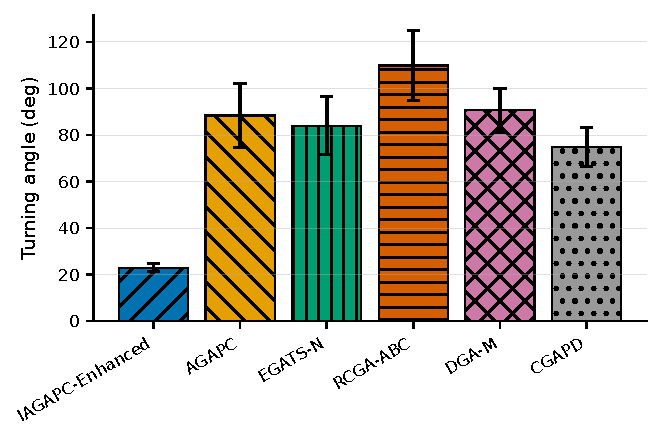
\includegraphics[width=\linewidth]{../figures/fig_turning_angle.pdf}
\caption{Turning angle by scheme (mean $\pm$ 95\% CI, $n{=}200$, 10 seeds).}
\label{fig:turning}
\end{figure}

One bar stands well below the rest. IAGAPC-Enhanced's whisker stops short
of every baseline whisker, which happens on no other chart in this
section, and the five baselines occupy a band from 74.8$^\circ$ to
109.9$^\circ$ while IAGAPC-Enhanced holds near 23$^\circ$.

\subsection{Energy Efficiency}

Unlike smoothness, energy efficiency depends on the whole network stack, 
routing, contention, and duty-cycling all feed into packets delivered per
joule. Table~\ref{tab:energy} gives this ratio over the same
configuration.

\begin{table}[t]
\centering
\caption{Energy efficiency by scheme (packets/J, mean $\pm$ 95\% CI, $n{=}200$, 10 seeds).}
\label{tab:energy}
\begin{tabular}{lc}
\toprule
Scheme & Packets / Joule \\
\midrule
EGATS-N & 2.52 $\pm$ 1.10 \\
AGAPC & 3.13 $\pm$ 2.33 \\
IAGAPC-Enhanced & 4.33 $\pm$ 1.98 \\
RCGA-ABC & 5.16 $\pm$ 6.41 \\
CGAPD & 8.29 $\pm$ 6.38 \\
DGA-M & 8.39 $\pm$ 7.84 \\
\bottomrule
\end{tabular}
\end{table}

Confidence intervals overlap substantially across all six schemes. DGA-M's
alone spans 0.55 to 16.22 packets/J. At this sample size the six schemes
are statistically indistinguishable on this metric. We report that rather
than selecting the numerically highest mean as a headline claim.

\begin{figure}[H]
\centering
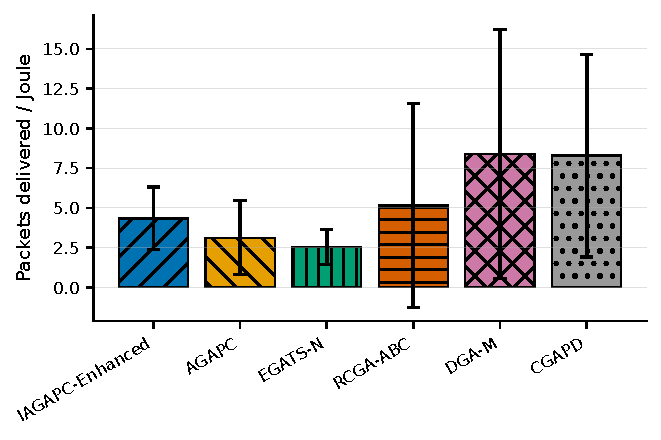
\includegraphics[width=\linewidth]{../figures/fig_energy_efficiency.pdf}
\caption{Energy efficiency by scheme (packets/J, mean $\pm$ 95\% CI, $n{=}200$, 10 seeds).}
\label{fig:energy}
\end{figure}

\subsection{Delivery Ratio, Throughput, and Delay}
\label{sec:pdr}

PDR ranged 0.041\% (EGATS-N) to 0.136\% (DGA-M) with CIs overlapping
between every pair. Throughput and delay show the same pattern. Neither
metric separates the six schemes at this sample size, which we report
directly rather than an unsupported ranking. Section~\ref{sec:losses}
explains why absolute delivery is low across all six at once. The
more informative reading of this result than any relative ordering. We
tabulate the underlying per-scheme means and 95\% CIs in
Table~\ref{tab:pdrthr}.

\begin{table}[t]
\centering
\caption{Delivery ratio, throughput, and delay by scheme (mean $\pm$ 95\% CI, $n{=}200$, 10 seeds).}
\label{tab:pdrthr}
\begin{tabular}{lccc}
\toprule
Scheme & PDR (\%) & Throughput (kbps) & Delay (s) \\
\midrule
IAGAPC-Enhanced & 0.071 $\pm$ 0.031 & 0.058 $\pm$ 0.026 & 11.86 $\pm$ 15.21 \\
AGAPC & 0.051 $\pm$ 0.038 & 0.042 $\pm$ 0.031 & 11.50 $\pm$ 14.90 \\
EGATS-N & 0.041 $\pm$ 0.018 & 0.034 $\pm$ 0.015 & 6.16 $\pm$ 5.43 \\
RCGA-ABC & 0.084 $\pm$ 0.105 & 0.069 $\pm$ 0.086 & 8.87 $\pm$ 16.98 \\
DGA-M & 0.136 $\pm$ 0.127 & 0.112 $\pm$ 0.105 & 19.77 $\pm$ 23.77 \\
CGAPD & 0.135 $\pm$ 0.104 & 0.111 $\pm$ 0.085 & 41.62 $\pm$ 35.41 \\
\bottomrule
\end{tabular}
\end{table}

\begin{figure}[H]
\centering
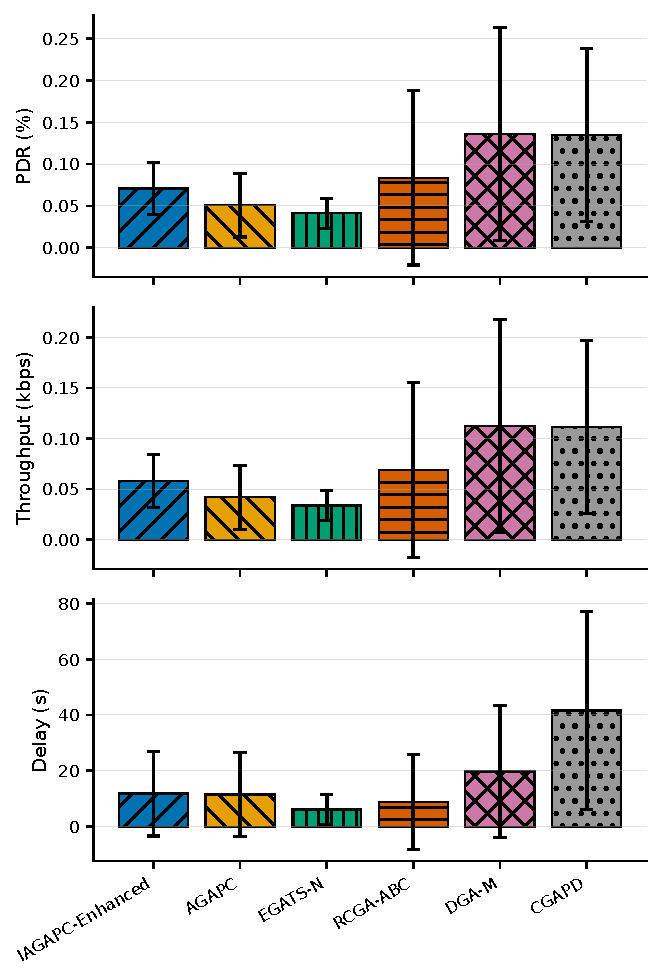
\includegraphics[width=0.8\linewidth]{../figures/fig_pdr_thr_delay.pdf}
\caption{PDR, throughput, and delay by scheme (mean $\pm$ 95\% CI, $n{=}200$, 10 seeds).}
\label{fig:pdrthr}
\end{figure}

The plotted intervals repeat what Table~\ref{tab:pdrthr} lists
numerically: on each of the three panels, all six schemes overlap. CGAPD's
delay interval is the extreme case at 41.62 $\pm$ 35.41\,s, wide enough to
swallow most of the other point estimates. What changes from panel to
panel is the absolute scale, not the separation between schemes.

\subsection{Network Lifetime: Evaluation Gap}
\label{sec:lifetime}

The energy recalibration needed (Section~\ref{sec:setup}) for nodes to
realistically survive showed full sink tour that eliminated node mortality
within the simulated horizon, across all 60 runs, FND/HND/LND are all
unreached. We report no values for them, since none exist at this
horizon. An evaluation gap requiring a longer simulated duration
to close, not a finding about scheme behavior.

\subsection{Loss Breakdown, PHY-Layer Contention, and Limitations}
\label{sec:losses}

Absolute delivery performance is low across every scheme in this
evaluation (Section~\ref{sec:pdr}), and we traced why rather than leaving it
unexplained. Table~\ref{tab:loss} decomposes 610{,}094 relay-hop-level
transmissions, aggregated across all 60 runs of this configuration, by
outcome.

\begin{table}[t]
\centering
\caption{Aggregate loss breakdown, 60 runs (6 schemes $\times$ 10 seeds), as \% of 610{,}094 relay-hop sends.}
\label{tab:loss}
\begin{tabular}{lrr}
\toprule
Outcome & Count & \% \\
\midrule
Received at sink & 630 & 0.10\% \\
Greedy-forwarding dead end & 129{,}053 & 21.15\% \\
Leaf buffer overflow (drop-oldest) & 30{,}100 & 4.93\% \\
Stranded, cluster head never sink-visited & 4{,}667 & 0.76\% \\
Stranded, cluster head visited but not yet flushed & 195 & 0.03\% \\
\bottomrule
\end{tabular}
\end{table}

\begin{figure}[H]
\centering
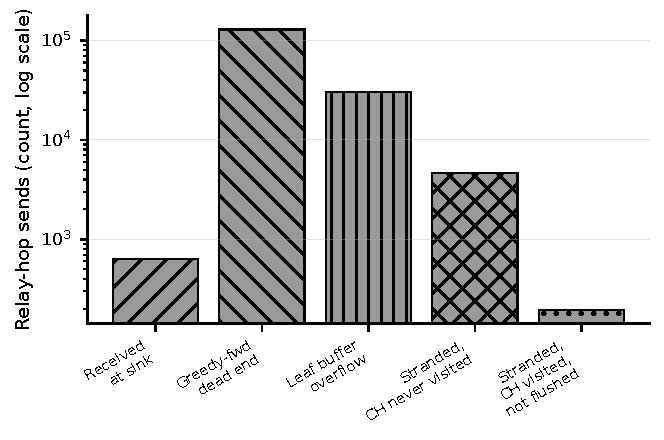
\includegraphics[width=\linewidth]{../figures/fig_loss_breakdown.pdf}
\caption{Loss breakdown by outcome, 60 runs aggregate (log scale; outcome
counts span 195 to 129{,}053).}
\label{fig:loss}
\end{figure}

The log axis is not cosmetic. Greedy-forwarding dead ends number 129{,}053
against 195 for the smallest stranded category, nearly three orders of
magnitude apart. A linear axis would compress every bar except the
dead-end and leaf-overflow ones onto the baseline. Those two outcomes take
most of the losses we can attribute. The 630 packets that reached the sink
form the second-shortest bar.

\sloppypar
These five outcomes cover roughly 27\% of relay-hop sends; the rest is
invisible to any application-layer counter. NS-3's own PHY-layer drop trace
explains why, it fires 7{,}754{,}706 times across the same 60 runs, over
twelve times the total sends. It counts every reception failure at every
radio in range, not only packets addressed to it. PHY-layer contention
among 200 nodes on one channel under greedy multi-hop relay is the
dominant loss mechanism, and it traces to a disclosed system-model
deviation: \texttt{WifiHelper} (IEEE 802.11b, lowest rate), not IEEE
802.15.4, not presented as equivalent. RTS/CTS plus the lowest data rate
cut PHY reception failures 32\% without resolving the underlying
contention. It is consistent with a property of the 802.11 contention
model at this density, not a tunable parameter. A narrowband CSMA-CA
802.15.4 PHY would not necessarily reproduce this severity, and we make no
claim it would. Absolute PDR, throughput, and delay here characterize this
WiFi-modeled layer under 200-node contention, not a real 802.15.4
deployment.

Two further disclosed limitations. Our current-times-airtime energy
accounting agrees with the classic rate-independent first-order model only
in a narrow data-rate band. At our low sensing rate, per-packet energy cost
runs roughly an order of magnitude above that formula's prediction. The proposed
energy figures are not interchangeable with classically-computed lifetime
results. Separately, duty cycling's isolated contribution to
Table~\ref{tab:energy} could not be validated. It disables the
only code path that transmits anything, giving a degenerate zero-packet
comparison, not a meaningful ablation. Neither limitation confounds the
six-scheme comparison itself. Every run applied identical configuration
across all six, so both bound only the interpretation of absolute
magnitudes.

Across Tables~\ref{tab:turning}, \ref{tab:energy}, and \ref{tab:pdrthr}:
turning angle separates cleanly (IAGAPC-Enhanced vs. all five baselines,
non-overlapping CIs); PDR, throughput, delay, and energy efficiency that do not
(overlap 95\% CIs). Network lifetime is unevaluated at this horizon
(Section~\ref{sec:lifetime}); Table~\ref{tab:loss} (Section~\ref{sec:losses})
traces why absolute delivery is low across all six.

\section{Conclusion and Future Work}
\label{sec:conclusion}

We proposed IAGAPC-Enhanced, a GA for mobile-sink trajectory planning
adding spline densification and kinematic-feasibility enforcement to
adaptive operator control and a diversity-restart mechanism, and evaluated
it against five baselines under one shared clustering, relay, and energy
substrate in ns-3.45.

One finding is clean and statistically separated across ten seeds,
IAGAPC-Enhanced's trajectories turn substantially less sharply than any
baseline's (22.99$^\circ$ vs. 74.81--109.89$^\circ$, non-overlapping CIs),
directly attributable to its spline-densification and
kinematic-feasibility mechanisms. PDR, throughput, delay, and energy
efficiency do not separate the six schemes at this sample size, and we
report that rather than an unsupported ranking. Absolute delivery is low
across all six, traced (Section~\ref{sec:losses}) to PHY-layer contention
among 200 nodes on one WiFi-modeled channel. This results in a disclosed deviation
from the IEEE 802.15.4 system model, not presented as equivalent to it. It
is identical across all six schemes, so it explains none of the (absent)
between-scheme difference.

Three limitations motivate future work: the WiFi-modeled link layer
(\texttt{LrWpanHelper} would place contention under the actual target radio
class), network lifetime unevaluated at this horizon, since the energy
recalibration needed for tour survival also eliminated mortality within it. And a single sink's hard coverage ceiling over a 200-node,
1000\,m$\times$1000\,m deployment, which a multi-sink extension would
relax, letting trajectory-quality differences surface in delivery metrics
where one sink's ceiling currently masks them.

\bibliographystyle{splncs04}
\bibliography{refs}

\end{document}